\chapter{Self-hosted Oracle Implementation} \label{chap:concl}

\section*{}

In this chapter I present a possible implementation of a multi-purpose self-hosted oracle. Multi-purpose since it will be able to query a requested API and return a specific value from the answer of that API, allowing to be used by several contracts which require different information and different sources. Self-hosted, as its code is available for anyone to copy and use for their own purpose and not having to rely on and oracle-as-a-service product by deploying their own version of the oracle.

As far as the author as searched, at the moment there is no clear explanation on how to implement your own oracle and therefore on how to power smart-contracts to query the web. Creating, therefore, a need for such a clear and detailed explanation as it will be presented in this section.

In principle, the described oracle is intended to be used by single entities or competing parties. Meaning, that it requires a list of predefined oracles and a predefined minimum quorum. Therefore, is not open to a community in which oracles can leave and join the network. The rationale behind this decision is that if it were to be open to a community the decision power in the final result would be dependent on who could launch the most oracles, solving this issue would require  the use of strategies, such as, proof-of-work which would become a different issue that the one the author is trying to solve.
In this setup, competing parties which may not trust each other, would be able to power their contracts by having each party launching one oracle, and therefore having all the same power of decision. Has the list of the oracles address is in the open on the oracle smart contract, there is no way for a party to cheat in their voting power.

\section{Oracle Overview}

The oracle compromises two main components, the on-chain oracle and the off-chain oracle. Figure \ref{fig:/figures/self-hosted-architecture} depicts the general architecture and a simplified version of the messages exchanged.

\begin{figure*}[t]
    \begin{center}
        \leavevmode
        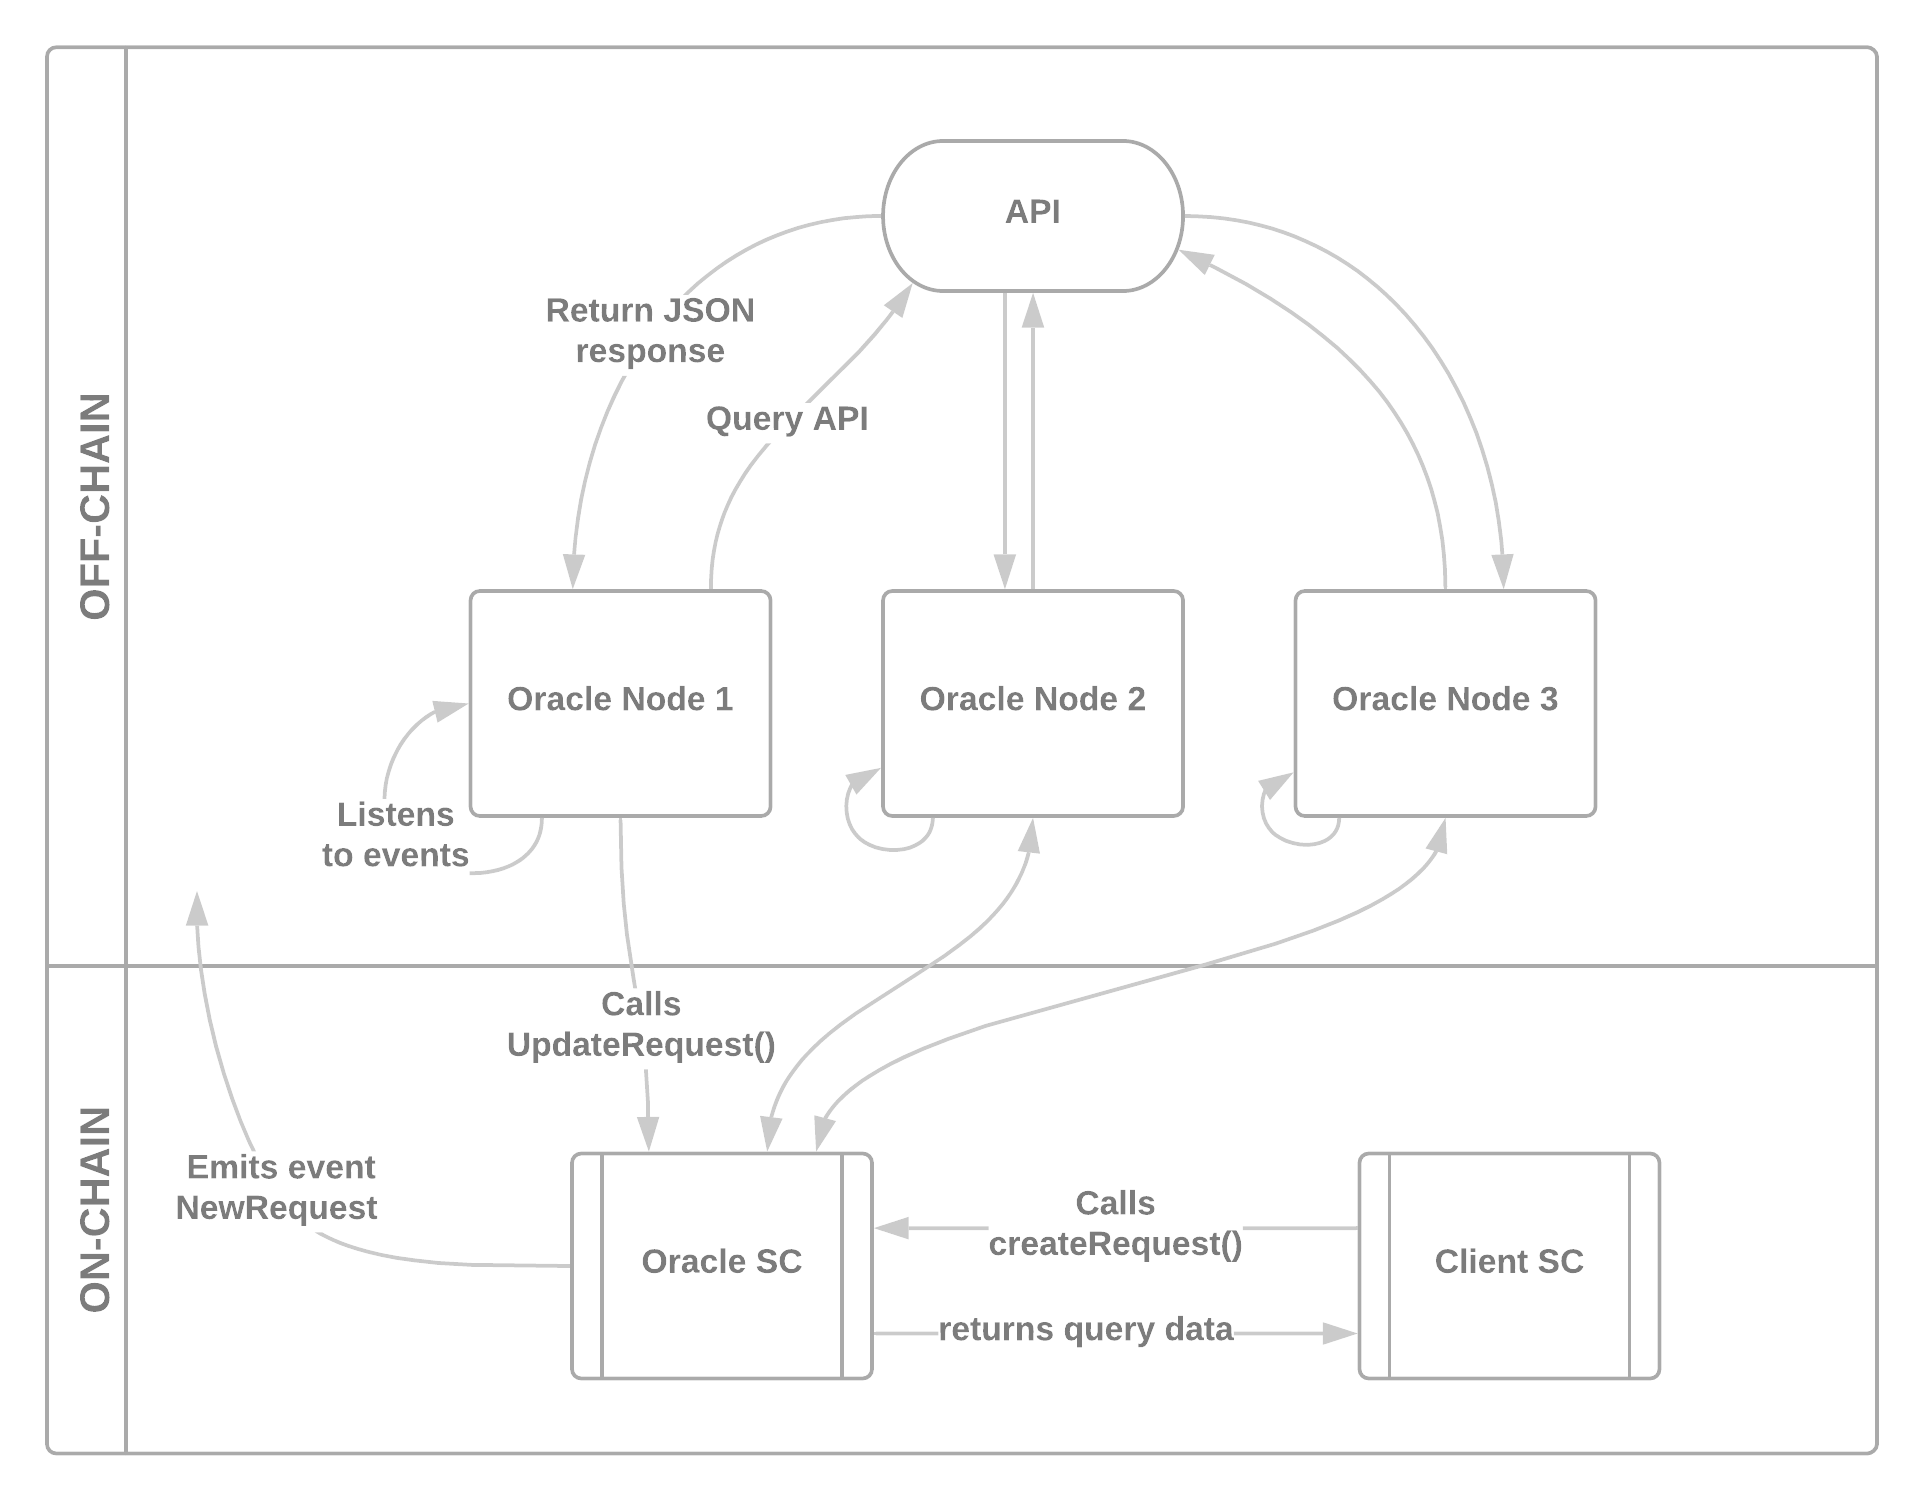
\includegraphics[width=1\textwidth]{figures/self-hosted-architecture.png}
        \caption{Self-hosted architecture.}
        \label{fig:/figures/self-hosted-architecture}
    \end{center}
\end{figure*}


The on-chain oracle is a smart contract that functions as a bridge between a client smart contract that needs information from the web and the oracle service that will query the web. This oracle has a whitelist of oracle addresses which are trusted by the oracle to query the web and has the necessary functions to create events that will trigger API calls and reach a consensus and the necessary data structures to store the requests and the agreed answer.

The off-chain oracle, or oracles, are services that continuously listen to specific events emitted by the oracle smart contract. Upon listening to a \textit{NewRequest} event query the specified API and key and return a single value to the smart contract by means of a new transaction.

This architecture allows for the use of several oracle nodes and the use of minimum voting quorums to achieve higher levels of trust, include more parties or increase service availability. However, the higher the number of oracles the higher the cost per transaction. Table \ref{oracle-query-cost} shows the cost of each query in euro using different numbers of oracles\footnote{Each test was composed of 110 requests using the same settings (Gas Price of 20 Gwei) except for the number of oracles. The result shown is the average cost of each request.}.


\begin{figure}[H]
    \centering
    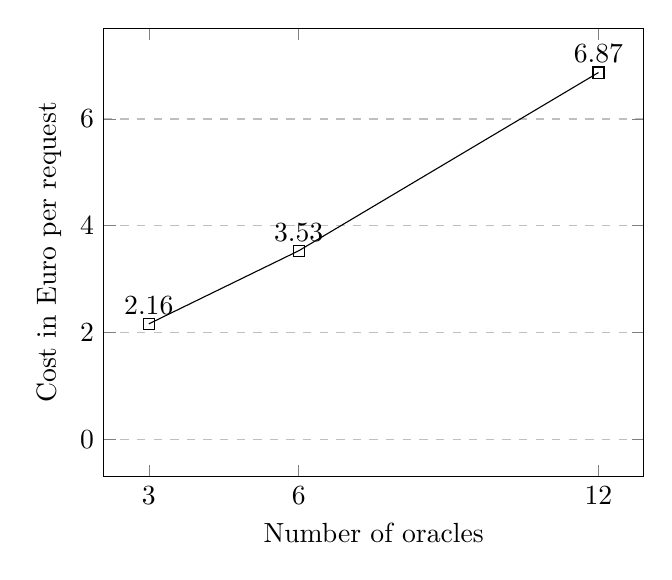
\begin{tikzpicture}
        \begin{axis}[
                xlabel={Number of oracles},
                ylabel={Cost in Euro per request},
                xtick=data,
                x tick label style={
                        /pgf/number format/1000 sep=},
                xmin=3, xmax=12,
                ymin=0, ymax=7,
                ytick={0,2,4,6,8},
                ymajorgrids=true,
                grid style=dashed,
                enlargelimits=0.10,
            ]

            \addplot[
                mark=square, nodes near coords
            ]
            coordinates {
                    (3,2.16)(6,3.53)(12,6.87)
                };

        \end{axis}
    \end{tikzpicture}
    \caption{Cost per query using a consensus of 2/3,}{Queried Google Finance on the 22th of May, 2019.}
    \
    \label{oracle-query-cost}
\end{figure}

\section{Component analysis}


\subsection{On-Chain Oracle}

The on-chain oracle is a smart contract that has an array which stores the requests made to the contract. Hard-coded in the contract is the predefined minimum quorum, which is the minimum number of equal answers needed to trust in the declaration of a final result. This minimum quorum will be used in all requests to the contract. Also hard-coded are the white-listed addresses of oracles that the contract will accept transactions to update requests.

Having the addresses and minimum quorum hard-coded on the oracle smart contract is not a software anti-pattern but rather an imposition on the contract terms. Doing so allows all parties who depend on this oracle to previously know that the oracle will always query those addresses and therefore they cannot be later altered for the benefit of one or more parties.

The code for the on-chain oracle can be found in the appendix \ref{ap2:on-chain-oracle-code} and due to its small size can be easily interpreted. Nonetheless, an explanation of its logic is detailed bellow.

\subsubsection{Creating a request}

Initially the request structure \ref{code:request-struct} only contains the URL which will be queried by the off-chain oracle and the attribute to return in the json API response.

\begin{lstlisting}[language=Solidity, label=code:request-struct]
  struct Request {
    uint id;                            //request id
    string urlToQuery;                  //API url
    string attributeToFetch;            //json attribute (key) to retrieve in the response
    string agreedValue;                 //value from key
    mapping(uint => string) anwers;     //answers provided by the oracles
    mapping(address => uint) quorum;    //oracles which will query the answer (1=oracle hasn't voted, 2=oracle has voted)
  }
\end{lstlisting}

A client smart contract calls the public function \textit{createRequest}
passing the url to query and the attribute from the api response that it needs to retrieve. This will add a new request to the array of requests in the oracle smart contract, initializing the list of trusted off-chain oracles addresses, the quorum. This list is composed of the addresses of the accounts which are trusted to add their input by creating transactions to the on-chain oracle contract.

The mapping of each address to an unsigned int is initialized at one, due to the fact that by default a mapping contains all possible addresses initialized at zero. By marking an address at one we explicitly set the trusted addresses so that later we can filter messages whose sender was previously marked with one.

Finally, an the \textit{NewRequest} event \ref{code:newrequest-event} is emitted so as to alert the off-chain oracles of the existence of a new request.

\begin{lstlisting}[language=Solidity, label=code:newrequest-event]
    event NewRequest (
        uint id,
        string urlToQuery,
        string attributeToFetch
    );
\end{lstlisting}

\subsubsection{Reaching consensus}

Each off-chain oracle, upon listening to the \textit{NewRequest} event will query the specified API and call the \textit{updateRequest} function on the on-chain oracle contract passing the id of the request and the value it retrieved from the API. The calling of the function is done by means of inputing a new transaction on the blockchain addressed to the smart contract, this will make the requested information available on the blockchain to be used by the contract.

The on-chain oracle contract, will first check if the transaction came from the whitelisted oracle addresses and if so, mark, that for this specific request this oracle has inputed his answer. Then it will save the answer on the list of answers for that request and count how many answers are on the list that match the current answer. If the count matches the minimum quorum set on the contract, the oracle contract will set a final agreed value for that request, meaning that at least a specified minimum number of oracles have provided the same answer and so it can be trusted to be the correct answer. This will emit a \textit{UpdatedRequest} event \ref{code:updatedrequest-event} that will alert who ever made that request that an agreement was reached on its answer.


\begin{lstlisting}[language=Solidity, label=code:updatedrequest-event]
    event UpdatedRequest (
        uint id,
        string urlToQuery,
        string attributeToFetch,
        string agreedValue
    );
\end{lstlisting}


\subsection{Off-Chain Oracle}

The off-chain oracle is a service that continuously listens to the events emitted by the on-chain oracle contract, more specifically to the \textit{NewRequest} event.

For this proof-of-concept the author used a node.js service, detailed in Appendix \ref{ap3:off-chain-oracle-code}, which upon new requests queries a specified API and returns a value to the smart contract by means of a transaction.

In order to create theses transactions we connect to the Ethereum blockchain, using web3.js\footnote{https://web3js.readthedocs.io/en/1.0/}, an Ethereum JavaScript API, and configure the accounts which will add the transactions with the answers to the requests to the smart contract. These accounts are the ones whose account addresses are specified on the white-listed list of addresses on the on-chain oracle. The detailed code can be found on Appendix \ref{ap4:off-chain-ethereum-connection}.

The off-chain oracle is very versatile, as it can be written in any language, that is supported by the Ethereum API. It can be worked upon to easily integrate new APIs or further logic and features without requiring any changes to the smart contract, as long as it respects the contract callback requirements.

\section{Summary and Conclusions}

This oracle implementation, although simple, is a versatile proof-of-concept which can already be applied to multiple smart-contracts in different scenarios. Since it allows to query any supported API and to choose which field the client smart contract needs. Limited only in accepting requests to APIs which return an answer in JSON format and also to only one value, but those limitations are only from the developer perspective and can easily be removed. This allows to achieve a desired simplicity that does not constrain the current model to a single use case. Rather, the code base can be used to add new features accordingly to the needs of each case without requiring big and breaking changes, being therefore a great starting point tackling the biggest problems when creating an oracle from scratch.

Having explained the versatility of this approach we have to consider the cost and benefits of being self deployed. Firstly, by using a self-deployed oracle, no extra-fees\footnote{https://docs.oraclize.it/\#pricing} are charged by a third party. To be clear, the cost of making a request to an oracle-as-a-service provider is composed of making the call to the oracle smart-contract, meaning its execution, plus an extra-fee for using the service. Secondly, trust is maintained since we know exactly the code that is being executed, even in an environment of competing parties, since all parties can launch an oracle and have the same say in its final result. Thirdly, cost can be easily optimized, since cost in a smart-contract is proportional to the amount of executed code, the developer has full access to edit and improve the on-chain oracle contract and therefore can improve the cost of each transaction/answer from the oracle to the oracle contract. Whereas in a third-party service the on-chain oracle contract code is managed by the service to whom we pay. Since, third-parties usually use authenticity proofs as evidence of their honesty, those proofs will add an extra cost to the transaction. Nonetheless, there are some possible extra costs not taken into account in this analysis which are relate to the maintenance and deployment of the off-chain oracle, something that is taken care by the third-party oracle provider. However, this off-chain oracle can be also be self deployed or even if deployed on a cloud provider the cost is insignificant in comparison to the cost of each request made to the on-chain oracle as demonstrated in figure \ref{oracle-query-cost}.

All in all, this chapter alongside the corresponding Appendixes, \ref{ap2:on-chain-oracle-code} \ref{ap3:off-chain-oracle-code} \ref{ap4:off-chain-ethereum-connection}, present a simple but effective way of deploying a oracle platform, on-chain and off-chain, that easily abd cost effectively can support and further empower existing and future smart-contract scenarios with trust in mind.